% Simple Sectioned Essay Template
% LaTeX Template
%
% This template has been downloaded from:
% http://www.latextemplates.com
%
% Note:
% The \lipsum[#] commands throughout this template generate dummy text
% to fill the template out. These commands should all be removed when 
% writing essay content.
%
%%%%%%%%%%%%%%%%%%%%%%%%%%%%%%%%%%%%%%%%%

%----------------------------------------------------------------------------------------
%	PACKAGES AND OTHER DOCUMENT CONFIGURATIONS
%----------------------------------------------------------------------------------------

\documentclass[11pt]{article} % Default font size is 12pt, it can be changed here

\usepackage{geometry} % Required to change the page size to A4
\geometry{a4paper} % Set the page size to be A4 as opposed to the default US Letter

\usepackage{amsmath}
\usepackage{graphicx} % Required for including pictures
\usepackage{caption}
\usepackage{subcaption}
\usepackage{pythonhighlight}

\usepackage{float} % Allows putting an [H] in \begin{figure} to specify the exact location of the figure
\usepackage{wrapfig} % Allows in-line images such as the example fish picture

\usepackage{lipsum} % Used for inserting dummy 'Lorem ipsum' text into the template

\usepackage[square, numbers, comma, sort&compress]{natbib} % Use the natbib reference package - read up on this to edit the reference style; if you want text (e.g. Smith et al., 2012) for the in-text references (instead of numbers), remove 'numbers' 
\usepackage{braket}
\usepackage[utf8]{inputenc}
\usepackage[T1]{fontenc}
\usepackage{booktabs}

\linespread{1.5} % Line spacing

%\setlength\parindent{0pt} % Uncomment to remove all indentation from paragraphs

\graphicspath{{../Figures/}} % Specifies the directory where pictures are stored

\begin{document}

%----------------------------------------------------------------------------------------
%	TITLE PAGE
%----------------------------------------------------------------------------------------

%\begin{titlepage}

\newcommand{\HRule}{\rule{\linewidth}{0.5mm}} % Defines a new command for the horizontal lines, change thickness here

\begin{center} % Center everything on the page
\textsc{\LARGE Report on the Olympic History Dataset}\\[1.5cm] % Name of your university/college
\end{center}
\begin{flushright}
{\bf Author:} Pedro Leal
\end{flushright}


%----------------------------------------------------------------------------------------
%	INTRODUCTION
%----------------------------------------------------------------------------------------

\section{Preparing the Data}

The first step after loading the databases (athletes and {\it NOC} codes) is to get a sense of what the dataset is like. For this we first list the features in the dataset:

\begin{itemize}
\setlength\itemsep{0.05em}
    \item ID -  Unique number for each athlete
    \item Name - Athlete's name
    \item Sex - M or F
    \item Age - Integer
    \item Height - In centimeters
    \item Weight - In kilograms
    \item Team - Team name
    \item NOC - National Olympic Committee 3-letter code
    \item Games - Year and season
    \item Year - Integer
    \item Season - Summer or Winter
    \item City - Host city
    \item Sport - Sport
    \item Event - Event in which the athlete participated
    \item Medal - Gold, Silver, Bronze, or NA
\end{itemize}


Then we use Pandas methods for {\tt DataFrames}, {\tt describe()} and {\tt info()}. For the athletes dataframe it outputs:

\begin{table}[h]
\centering
\begin{tabular}{lrrrrr}
\toprule
{} &             ID &            Age &         Height &         Weight &           Year \\
\midrule
count &  271116 &  261642 &  210945 &  208241 &  271116 \\
mean  &   68248.95 &      25.56 &     175.34 &      70.70 &    1978.38 \\
std   &   39022.29 &       6.39 &      10.52 &      14.35 &      29.88 \\
min   &       1 &      10 &     127 &      25 &    1896 \\
25\%   &   34643 &      21 &     168 &      60 &    1960 \\
50\%   &   68205 &      24 &     175 &      70 &    1988 \\
75\%   &  102097.25 &      28 &     183 &      79 &    2002 \\
max   &  135571 &      97 &     226 &     214 &    2016 \\
\bottomrule
\end{tabular}
\caption{Descriptive Statistics for the numerical features in the dataset.}
\end{table}
\paragraph{\,}

The first stricking aspect of this early analysis is the maximum age of someone participating in the Olympics, at 97 years old! Also, the minimum age is quite strange (but not more than the already mentioned max age). The minimum and maximum values for Height and Weight is also striking. Before we proceed to analyse these particular cases to find out why they are here, let us use another tool, a Python library, built on top of the Pandas library, called Pandas Profiling. This generates an HTML file with all basic initial analysis of the dataset and allows for a better visualization of the characteristics of the dataset. The file generated is included in the attached documents with the name 'df\_pandas\_profiling\_OH.html'. 

The main concerns after analyzing the generated file are the missing data in "Height" and "Weight" features, both missing around $20\%$ of the data, and the number of redundant features in "Year", "Season" and "Games". We have the same observation in the "Age" feature: the highest value is 97 and additionally there are several entries above 50 years old. We should analyse them soon. Before we do that, though, we must first deal with the duplicates, with 1385 different instances repeated, and the missing data for "Age", "Height" and "Weight".

For checking the duplicates, one can use the create a new DataFrame containing only the entries with the duplicates. This will be done in two different ways: first we use {\tt athlete\_df[athlete\_df.duplicated(keep='first')]}, in order to check the report from the profile already obtained. Using the {\tt .shape} method we see that, indeed, there are 1385 different duplicated rows. Then, using {\tt athlete\_df[athlete\_df.duplicated(keep= False)]}, one can see that there are $1997$ total repeated rows, belonging to 515 different athletes. The sports in which the duplicates appear, obtained using {\tt duplicates\_df[' Sport'].value\_counts()}, is given in Table 2.

\begin{table}
\centering
\begin{tabular}{lr}
\toprule
Sport & Count  \\
\midrule
Art Competitions &   1857 \\
Sailing          &     74 \\
Cycling          &     64 \\
Equestrianism    &      2 \\
\bottomrule
\end{tabular}
\caption{Table with count of duplicate rows in each sport.}
\end{table}

In order to check if these were actually duplicate data, a narrow search was performed. For all but "Art Competitions" the repeated rows occurred in the same year (1900 for "Equestrianism" and "Sailing" and 1908 for "Cycling"), and upon closer inspection, unless two gold, silver and bronze medals were attributed to the same person on the same event, the data must in fact be duplicate. Therefore, the second occurrence in each was removed, with {\tt athlete\_df.drop(athlete\_df[(athlete\_df.Sport!='Art Competitions') \& (athlete\_df.duplicated())].index,axis=0,inplace=True)}.  

As for "Art Competitions" several years revealed this problem: 1924 (175 duplicates), 1928 (467 duplicates), 1932 (692 duplicates), 1936 (377 duplicates) and 1948 (146 duplicates), as seen in Table 3. However, one must be careful, since (upon checking the Wikipedia page on these artistic competitions, which I didn't know existed) in this competition participants were allowed to send in multiple works for the same category and were allowed to receive medals for more than one. One can see that some artists are featured two or more times for the same event, having however no evidence that these are not legitimate multiple-fold participations. One last check can be made: the medals awarded to the repeated rows, using {\tt duplicates\_df[(duplicates\_df["Sport"]=='Art Competitions')  \& (duplicates\_df['Medal']!='no\_medal')]}. It turns out that no medals were awarded to the "Art Competition" duplicated rows. For this reason together with the fact that artists were in fact allowed to have multiple works for competition, the duplicate rows will be kept in our dataset. These will not affect any conclusion taken regarding medal attribution. As a note, according to the Wikipedia page, these competitions ocurred in the Olympics Games between 1912 and 1948, agreeing with our dataset.

\begin{table}
\centering\begin{tabular}{lr}
\toprule
Year & Count  \\
\midrule
1932 &  1124 \\
1936 &   813 \\
1928 &   808 \\
1948 &   471 \\
1924 &   318 \\
1912 &    33 \\
1920 &    11 \\
\bottomrule
\end{tabular}
\caption{Table for the number of 'Art Competition' participants per year.}
\end{table}

After this, there was a need to remove redundant features. For this, the "Games" feature was split into "Season\_2" and "Year\_2" features and compared to the already existing features for these ("Year" and "Season"), to check for mismatches. Since there were none, "Games", "Season\_2" and "Year\_2" were removed, given that since we can get any "Games" feature by combining the other two.

Before getting to further explore the data, two important things must be done: one is to add a feature for the "Region" contained in the {\it noc\_regions.csv} file and the second is to add another feature containing the "Continent" to which each region belongs. The first is achieved through the merging of {\tt athlete\_df} and {\tt noc\_df} dataframes using {\tt pd.merge(athlete\_df,noc\_df[['NOC','region']],on='NOC',how='left')}. As for adding continents, despite the process within the Python script being the same, one must first have a dataframe that links each "NOC" to a particular continent. For that we have the file {\it raw\_continent.csv}, which has too many information and is therefore processed in {\it continent\_preprocess.py}, which takes only the relevant features from the initial data and saves it to the {\it continents.csv} file. In this step one must add any missing "NOC" and "Continent" features manually for some historical Olympic Committees that no longer exist. Additionally, North America is relabeled from "NA" to "NAm" because {\it Pandas} treats the former as a missing value, and we adde the continent class "Multi" for 'Individual Olympic Athletes' and 'Refugee Olympic Team' since they are not unknown and come from several continents. These two codes were used in several instances throughout history for people whose official International Olympic Committee did not participate or were fleeing from war at the time of the Games, respectively.

After this treatment, we prepare another profile. The only issue remaining is the amount of missing "Height" and "Weight" data. We will keep those as they are, since several analysis can be made about the participants with this missing features. In analysis where these features are needed, we will leave the missing values out.

After having done this, there should be no duplicate rows, no missing values apart from the "Height" and "Weight" ones and no redundant features. Thus, we are now able to make deeper analysis on this dataset.



\section{Data Visualization and Analysis}

\subsection{First Analysis}

Here, we start with the visual version of Table 1 in Figure 1.

\begin{figure}
    \centering
    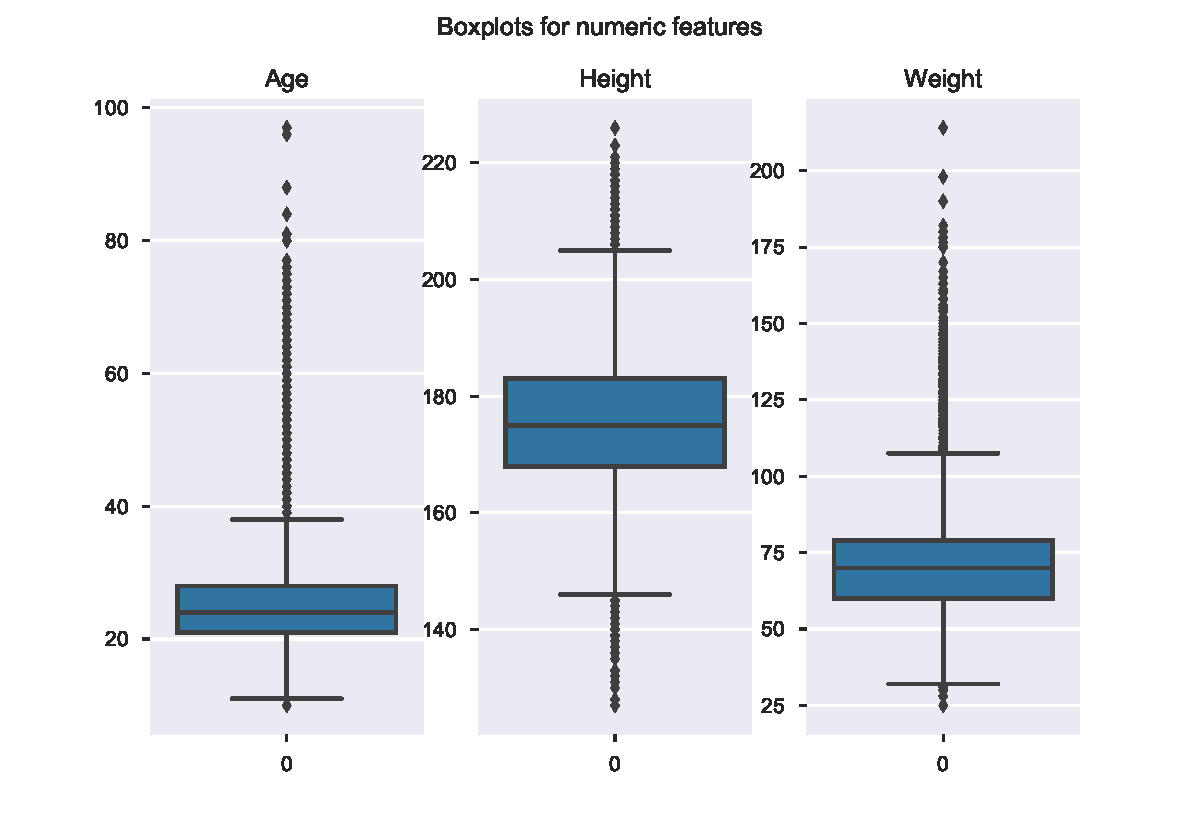
\includegraphics[scale=0.6]{Boxplot_numeric.pdf}
    \caption{Boxplots for the relevant numeric features.}
\end{figure}

As had been remarked earlier, there are in fact many outliers, the most striking ones being in the (old) 'Age' feature, with many participants having 50+ years. In Figure 2 we can see the that even when filtering by medals won, there are still people whose age is more than 50 years old who are in the data! We must discover more about these people.

\begin{figure}
    \centering
    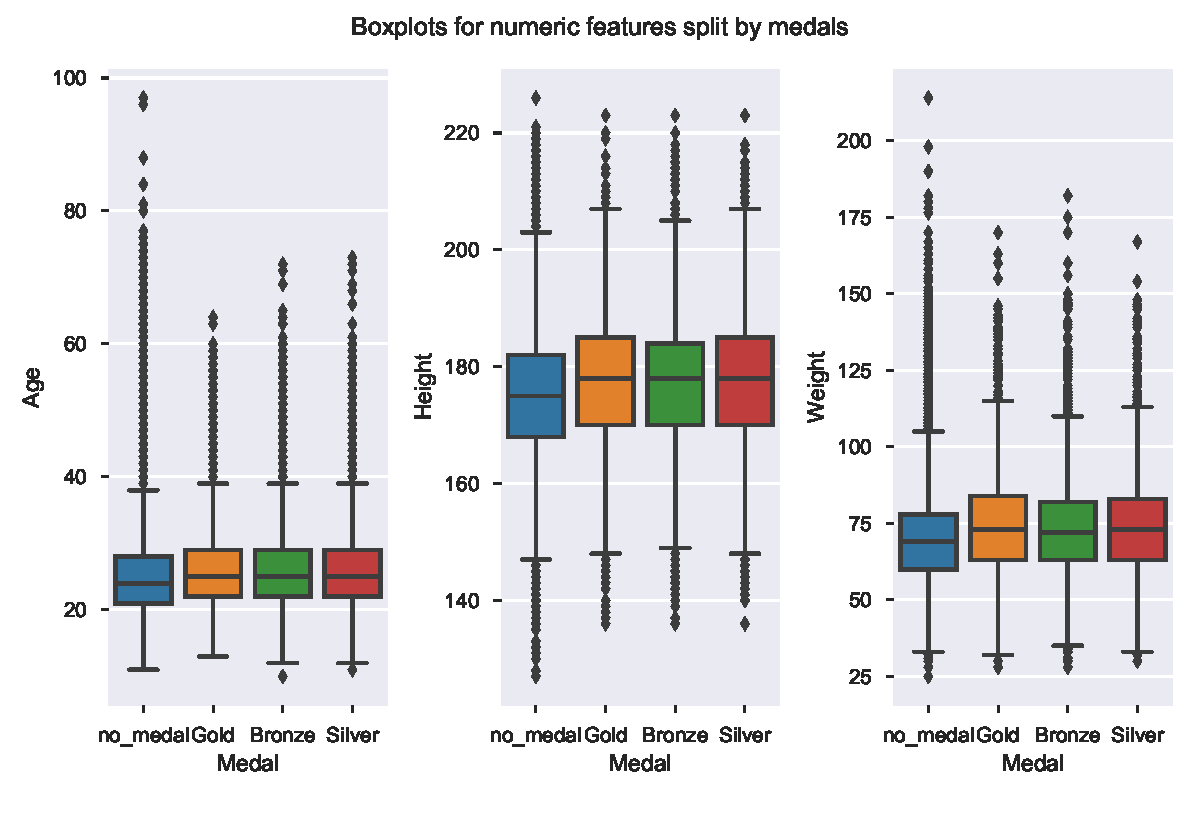
\includegraphics[scale=0.6]{Boxplot_numeric_medals.pdf}
    \caption{Boxplots for the relevant numeric features split by medal awarded.}
\end{figure}

When filtering the data for people whose age is 50+ (using {\tt athlete\_df[athlete\_df. Age>=50]}) we get 2213 entries divided by "Sport" according to Table 3. It turns out that most entries for which Age$>50$ are relative to an "Art Competitions" category, which features competition in architecture, painting, sculpture, literature and music.


\begin{table}
\centering
\begin{tabular}{lrrrr}
\toprule
Sport &  Participants &  Gold & SIlver & Bronze\\
\midrule
Art Competitions  &   1104 &      8 &     16 &     13 \\
Shooting          &    464 &     13 &     18 &     19 \\
Equestrianism     &    299 &     22 &     14 &     17 \\
Sailing           &    174 &     17 &     15 &     13 \\
Archery           &     73 &     11 &     15 &      8 \\
Fencing           &     49 &      1 &      2 &      0 \\
Rowing            &     10 &      0 &      3 &      0 \\
Bobsleigh         &      6 &      0 &      0 &      0 \\
Curling           &      5 &      2 &      2 &      0 \\
Golf              &      3 &      0 &      0 &      1 \\
Table Tennis      &      3 &      0 &      0 &      0 \\
Alpine Skiing     &      3 &      0 &      0 &      0 \\
Luge              &      2 &      0 &      0 &      0 \\
Polo              &      2 &      0 &      0 &      0 \\
Athletics         &      2 &      0 &      0 &      0 \\
Skeleton          &      2 &      0 &      0 &      0 \\
Roque             &      2 &      1 &      1 &      0 \\
Speed Skating     &      2 &      0 &      0 &      0 \\
Croquet           &      2 &      1 &      0 &      1 \\
Modern Pentathlon &      1 &      0 &      0 &      0 \\
Figure Skating    &      1 &      0 &      0 &      0 \\
Motorboating      &      1 &      0 &      0 &      0 \\
Alpinism          &      1 &      1 &      0 &      0 \\
Wrestling         &      1 &      0 &      0 &      0 \\
Diving            &      1 &      0 &      0 &      0 \\
\midrule
Total             & 2213 & 77 & 86 & 72 \\
\bottomrule
\end{tabular}
\caption{Number of entries by Sport for Age$\geq$ 50.}
\end{table}

Let us um this in a nicer way in Figure 3.

\begin{figure}
    \centering
    \includegraphics[scale=0.6]{Medal_Count_50.pdf}
    \caption{Countplots for medals awarded to people over 50 top 5 Sports.}
\end{figure}

\begin{figure}
    \centering
    \includegraphics[scale=0.6]{Gold_medal_Count_50.pdf}
    \caption{Countplots for gold medals awarded to people over 50 top 5 Sports.}
\end{figure}

It is then possible to see that most of the medals awarded to people over 50 are for sports with relative low effort. However, two of the participations were from Athletics and one for Wrestling. Let us get the full information on those three people and summarize it in Table 5. We can see that both men in "Athletics" participated in long distance runs, as opposed to short distances, which are usually reserved for younger people.

\begin{table}
\begin{tabular}{lrllrrrllrlllllll}
\toprule                        
Name &   Age &     NOC &  Year &                                      Event  \\
\midrule
Alexander Harold "Alex" Oakley &  50.0 &    CAN &  1976 &            Athletics Men's 20 kilometres Walk  \\
Hugo Anton Toeppen &  50.0 &        USA &  1904 &     Wrestling Men's Welterweight, Freestyle  \\
Percival "Percy" Wyer &   52.0 &      CAN &  1936 &                      Athletics Men's Marathon  \\
\bottomrule
\end{tabular}
\caption{Some participants over 50 years old.}
\end{table}

Finishing this section, we should get a closer look at the athletes who are younger than 15. Looking at Figure 5, one can see that these athletes are mostly female, with relatively little success in getting medals. Using the {\tt value\_counts()} method, we see that most of these participate in Swimming ($42.71\%$) and Gymnastics ($39.05\%$).

\begin{figure}
    \centering
    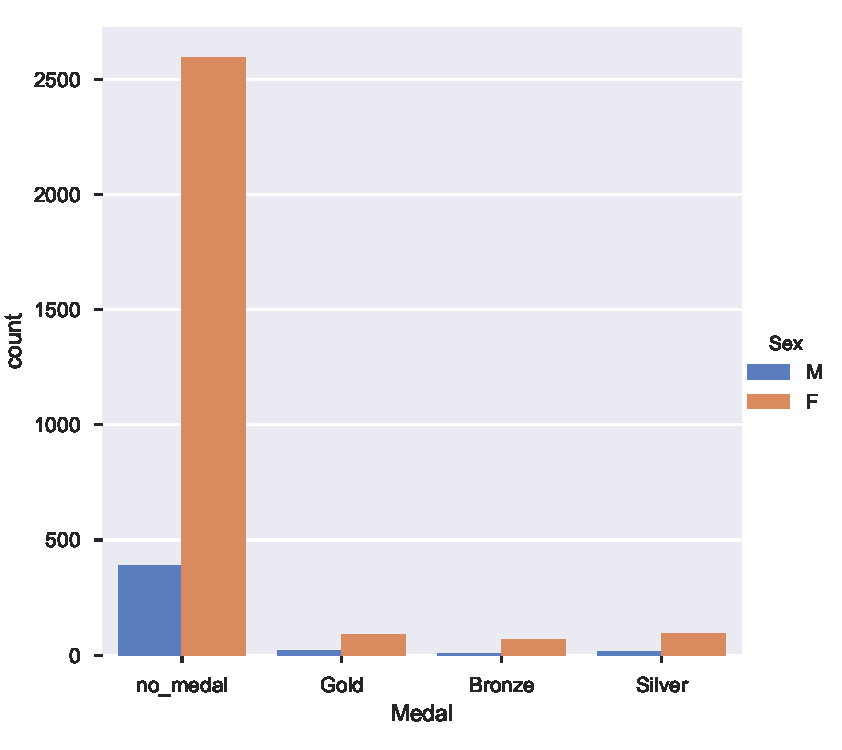
\includegraphics[scale=0.8]{Countplot_under_15.pdf}
    \caption{Participants under 15.}
\end{figure}

Still related to age, looking at Figure 6, it is possible to take several conclusions: first, women who participate in the Olympics tend to be younger than men; second, Sport can have an impact on the Age distribution of its athletes; and third, there is no significant difference in age between the different groups with regards to medals.

\begin{figure}
    \centering
    \begin{subfigure}{.5\textwidth}
    \hspace{-17mm}
    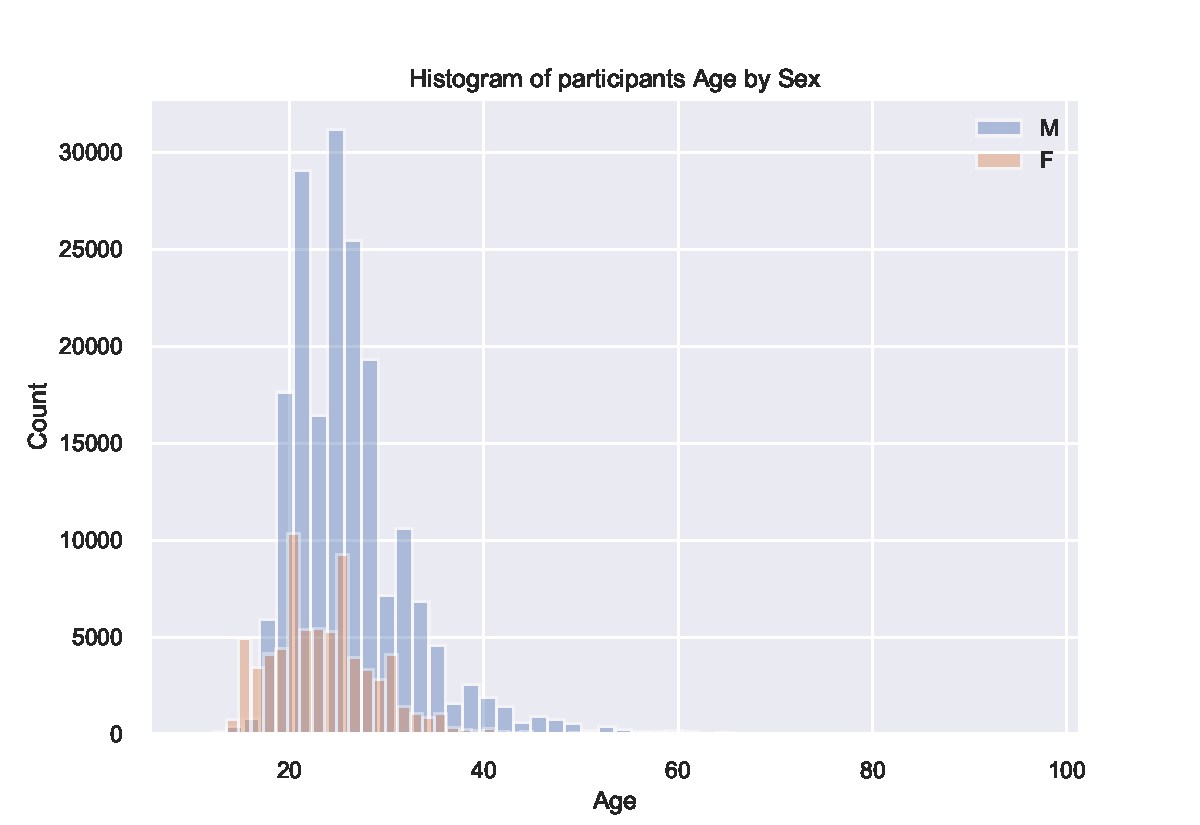
\includegraphics[scale=0.45]{Age_hist_by_Sex.pdf}
    \end{subfigure}%
    \begin{subfigure}{.5\textwidth}
    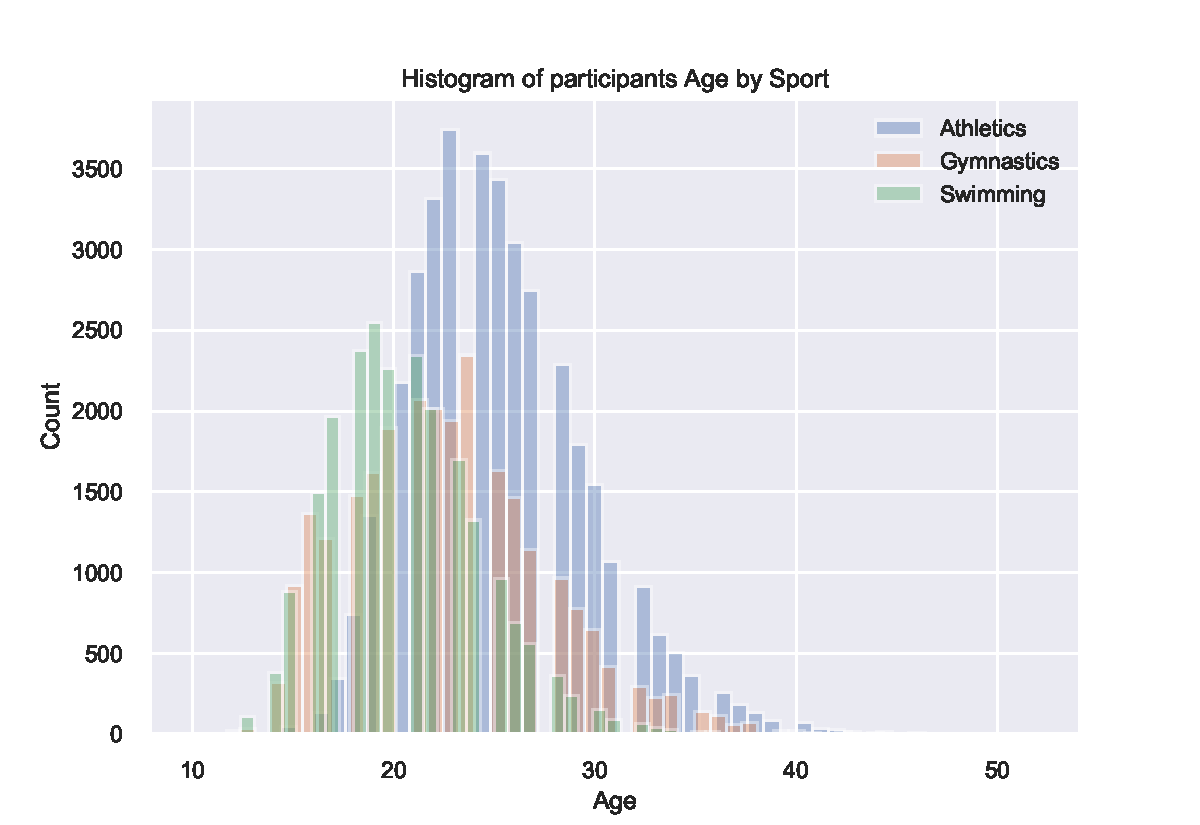
\includegraphics[scale=0.45]{Age_hist_by_Sport.pdf}
    \end{subfigure}
    \begin{subfigure}{.5\textwidth}
    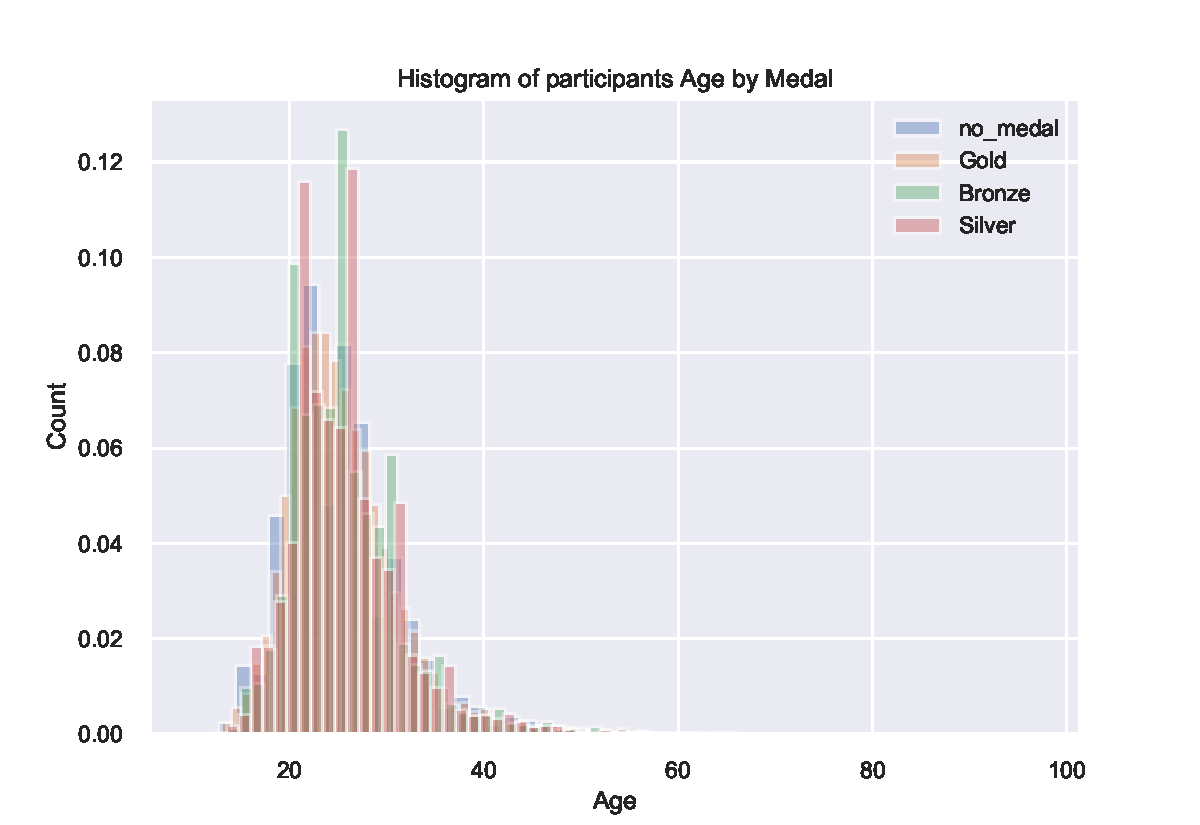
\includegraphics[scale=0.5]{Age_hist_by_Medal.pdf}
    \end{subfigure}
    \caption{Histograms of Age.}
\end{figure}

The same conclusions can be reached to the "Height" variable, as can be seen in Figure 7, where men are taller than women, there is a significant difference between the listed sports and there seems to be no correlation between medal awarding and height.

\begin{figure}
    \centering
    \begin{subfigure}{.5\textwidth}
    \hspace{-17mm}
    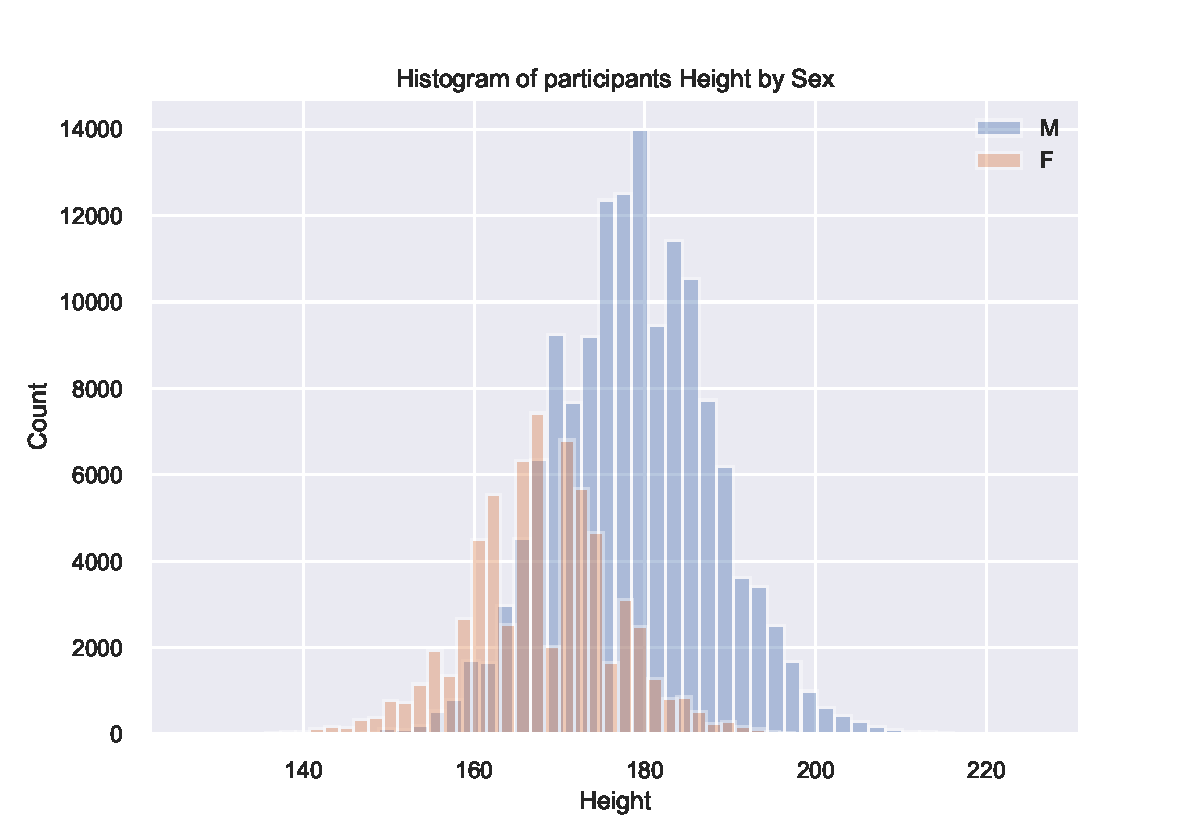
\includegraphics[scale=0.45]{Height_hist_by_Sex.pdf}
    \end{subfigure}%
    \begin{subfigure}{.5\textwidth}
    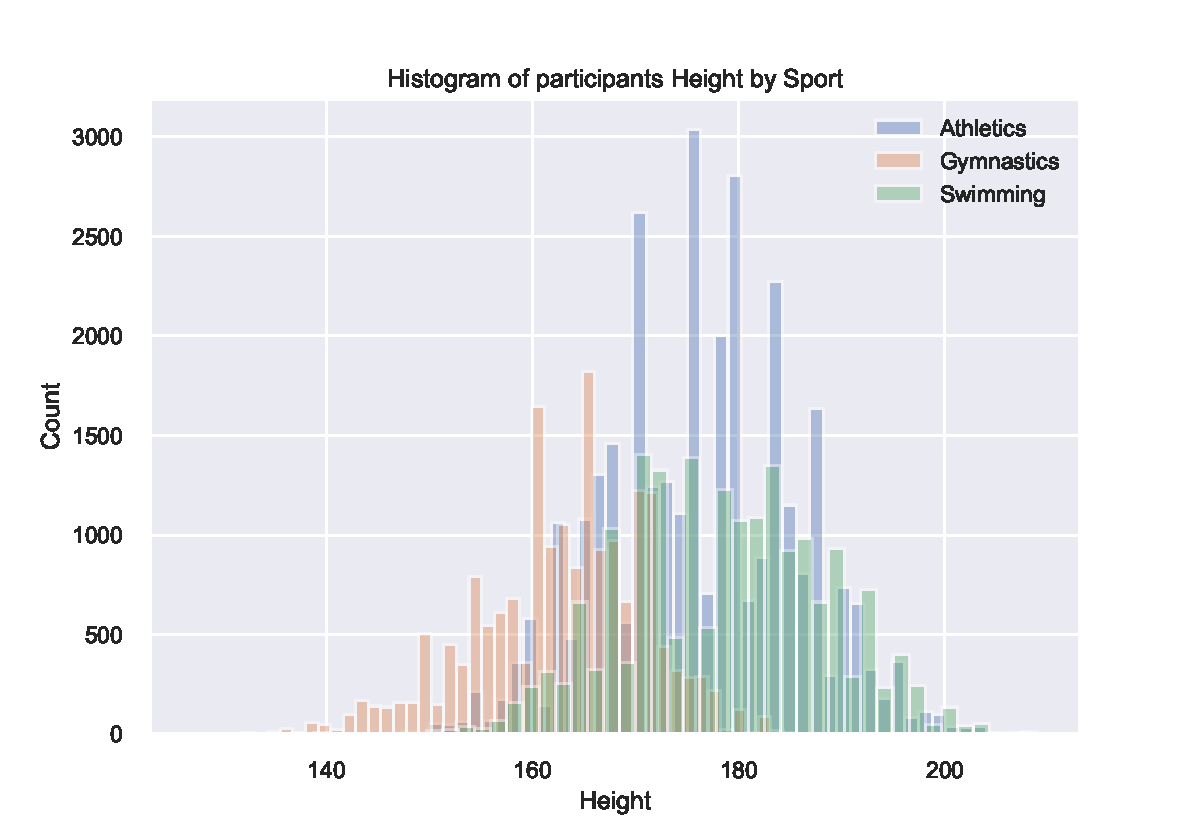
\includegraphics[scale=0.45]{Height_hist_by_Sport.pdf}
    \end{subfigure}
    \begin{subfigure}{.5\textwidth}
    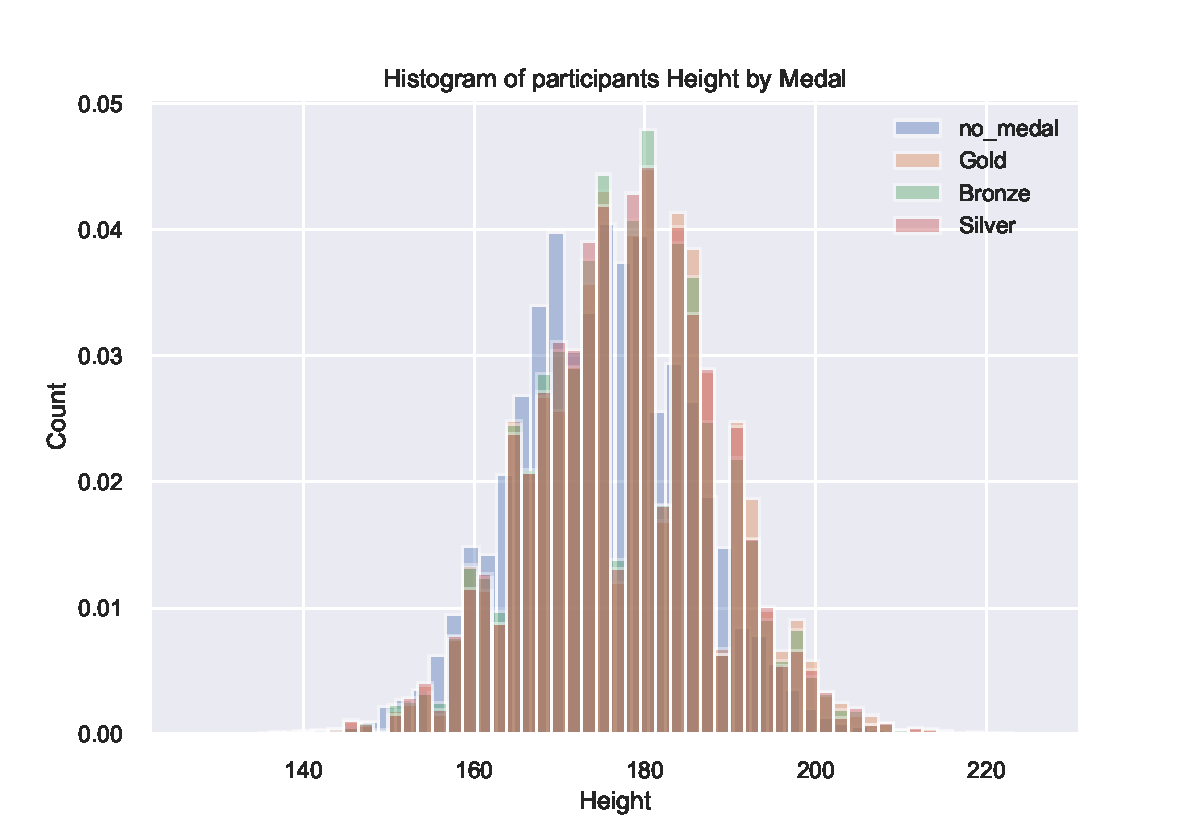
\includegraphics[scale=0.5]{Height_hist_by_Medal.pdf}
    \end{subfigure}
    \caption{Histograms of Height.}
\end{figure}

In order to finish the analysis of the numeric variables, let us see the relationship between "Height" and "Weight", as presented in Figure 8. We can clearly see a correlation between these two variables. Furthermore, women seem to be lighter and shorter than men. This correlation between features can be easily seen by using a heatmap, as in Figure 9, with a Pearson correlation coefficient of 0.8. This allows us to deduce that the behaviour we observed in Figure 7 generalizes to the "Weight" feature. In fact, this can be seen in the attached documents ({\it Weight\_hist\_by\_feature.pdf}).

\paragraph{Note} The histograms were produced using the function {\tt histograms}, whose definition is in the code below. This was used to plot histograms features grouped by classes of some other feature in the dataframe.

\begin{python}
def histograms(dataframe,feature,feature_to_group,classes_to_keep,same_hist=True,show=False,norm=False,distinguish_title=''):
    """

    This function plots histograms for a certain 'feature', making a separate histogram for each class in
    'feature_to_group'. One chooses the 'classes_to_keep' from the classes of 'feature_to_group'.

    If 'same_hist' is True, then all classes will be ploted in the same histogram; if False, then a subplot is created for each class.
    If 'show' is False, the Figure will be save; if True it will additionally be shown as the code runs.

    """
\end{python}

\begin{figure}
    \centering
    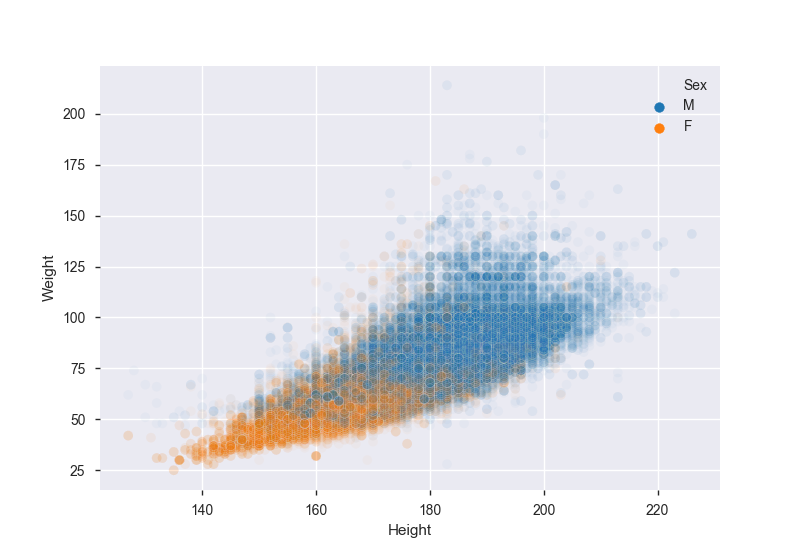
\includegraphics[scale=0.8]{Scatter_Height_Weight.png}
    \caption{Scatterplot of Height and Weight divided by Sex.}
\end{figure}

\begin{figure}
    \centering
    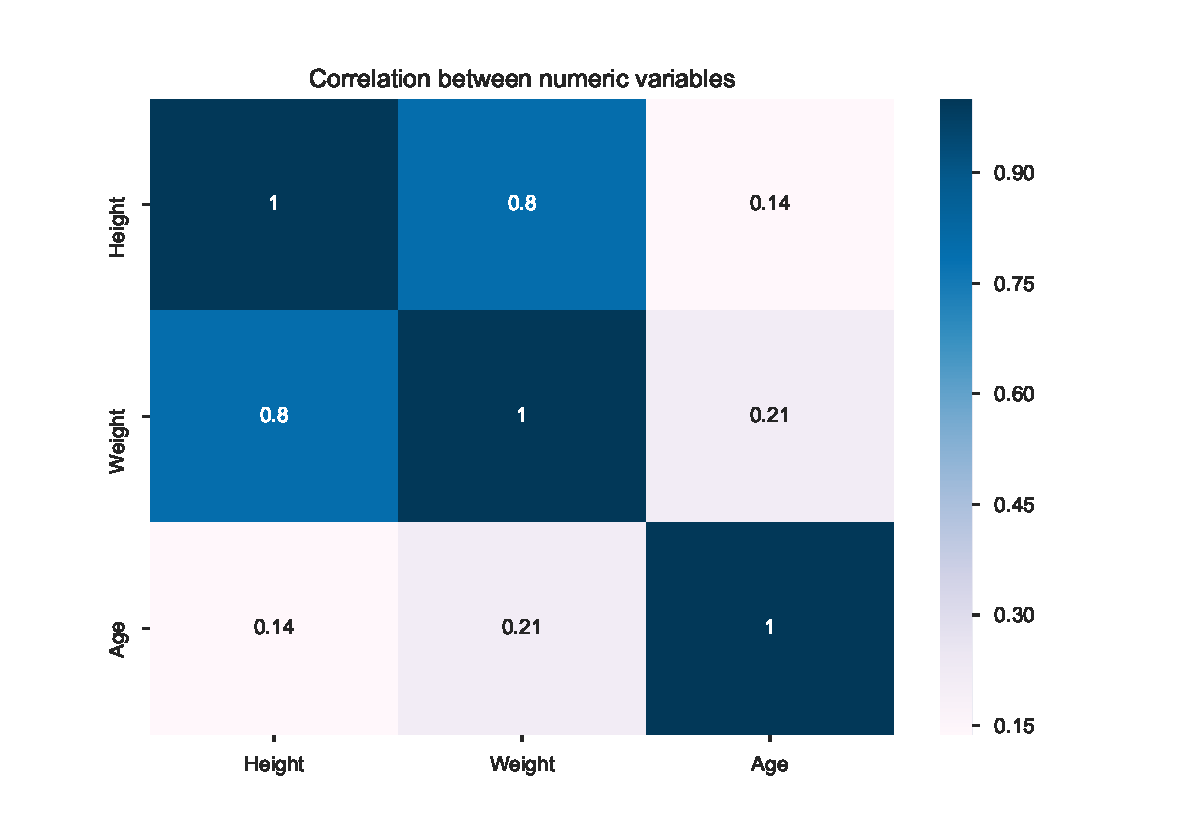
\includegraphics[scale=0.6]{Corr_heatmap.pdf}
    \caption{Heatmap of correlations.}
\end{figure}

\subsection{Time Dependent Analysis}

Now that we have explored the dataset and created visualizations that allows us to extract some information from it, let us see how some aspects of the Olympics Games evolved with time. Starting with the number of participants, we can see in Figure 10 a) that this number has been increasing since the inception of the modern Games in 1896, with a few exceptions: 1932, 1956, 1980 and then every other year since 1992. This may be explained by these being the first games after the Great Depression (1929). Looking at Figure 10 b) we can see that there was a decrease in both Summer and Winter Olympics.

\begin{figure}
    \centering
    \begin{subfigure}{1\textwidth}
    \centering
    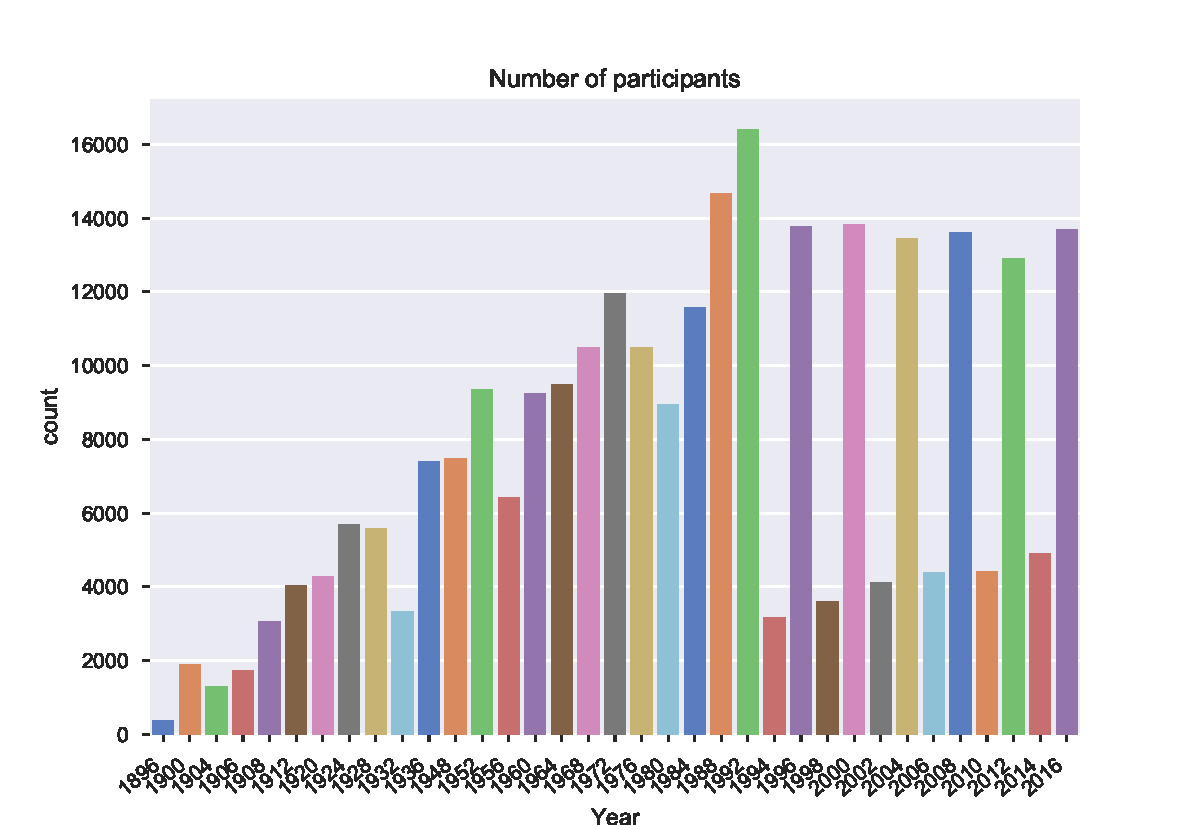
\includegraphics[scale=0.65]{Participants_year.pdf}
    \subcaption{Total participants.}
    \end{subfigure}
    \begin{subfigure}{1\textwidth}
    \centering
    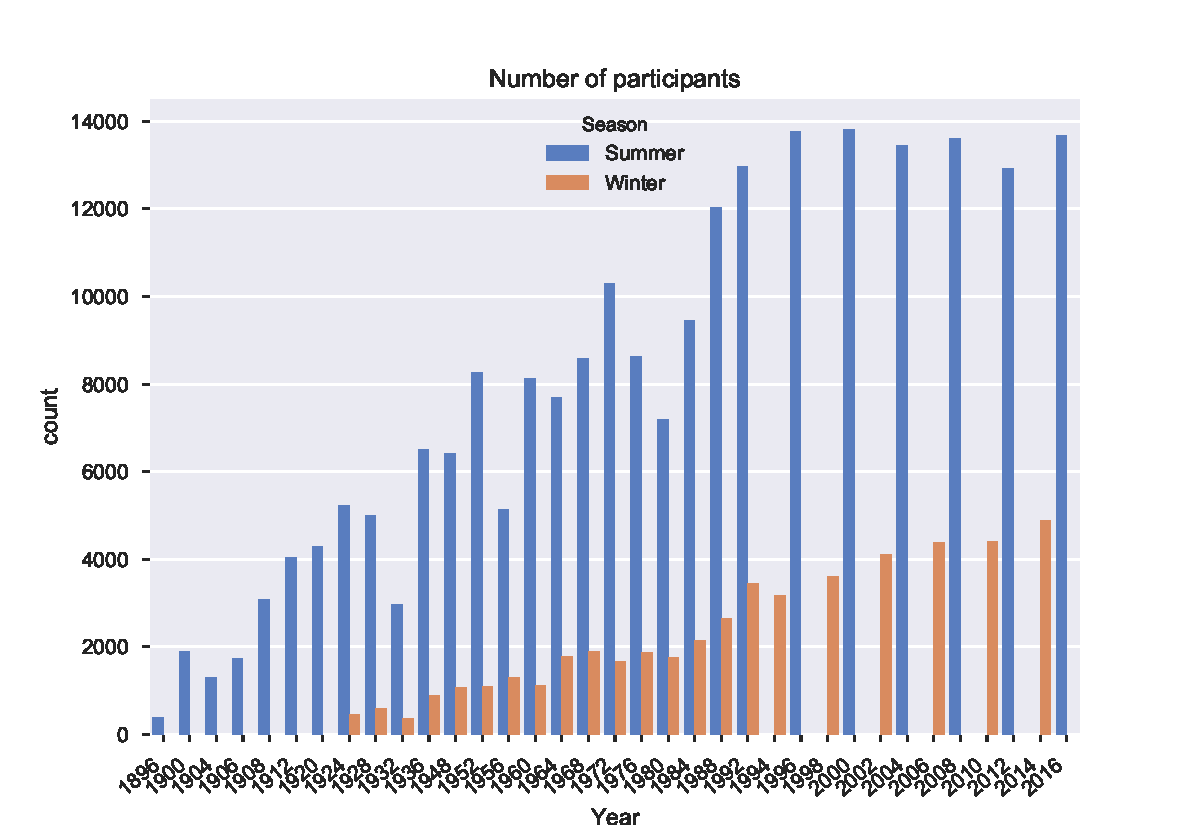
\includegraphics[scale=0.65]{Participants_year_season.pdf}
    \subcaption{Participants by Season.}
    \end{subfigure}
    \caption{Number of participants in the Olympics Games since 1896.}
\end{figure}

The decrease in 1956 can be attributed to a number of boycotts (China, Egypt, Iraq, Lebanon, the Netherlands, Spain, and Switzerland) because of different reasons, but all of them political. In 1980 and in 1984 the US and the Soviet Union, respectively boycotted the Olympics, being a possible reason for the decrease in participants. From 1992 onwards the change in the number of participants every two years can be explained by looking at Figure 10 b) alone: the Summer and Winter Olympics were separated, thus leading to a decrease in the total number of athletes in each of them (being that the Winter ones have fewer athletes in general). 



Another important analysis to make is related to the participation of women in the Olympics. Figure 11 indicates that the number of women participating has been constantly increasing (apart from 1956 and 1984, which were problematic years as explained above) and although not yet equal in number to men, are approaching equality, both in Summer and Winter Games. But how about the number of Gold, Silver and Bronze medals for women? We can see in Figure 12 that the number of any one of the medals awarded to women has been rising and it's now near equality with the men counterparts. This should not be surprising because in most sports women and men compete separately, so the amount of medals scales with the number of players of each gender, thus it being increasing for women in a nearly identical fashion as the number of women increases, as seen in Figure 11. 

\section{Time Independent Analysis}

Proceeding with the analysis, it would be interesting to see how the number of participants and medalists are distributed across continents. First, let's check which continent has more participants. This leads us to Figure 13 a), we can see that, over the years the continent with an overwhelming majority of athletes come from Europe, with North America and Asia following and the least athletes coming from Africa and Oceania. But how about the number of medals given to athletes from each of the continents? In Figure 13 b) we see that, not surprisingly, Europe has the most medals, but it seems that North America has proportionally more medals than Europe! Let us inspect the numbers. Analyzing Table 6 one can see that, indeed North America has a higher proportion of medals than any other continent, at 0.20 followed by Europe and Oceania, at 0.16 and 0.15, respectively.

Before proceeding, we shoul take a closer inspection at the athletes from non-continent regions, labeled here as "Multi" or "UNK". The former have 106 athletes: 94 from the "NOC" {\it IOA} for  Independent Olympic Athletes and 12 from {\it ROT} from the Refugee Olympic Team. All the athletes from the {\it ROT committee} are from 2016, which is verified upon checking the Wikipedia page for this team. It was fromed in 2016 for the athletes who were fleeing their country due to war, mainly in the Middle East. As for the {\it IOA} athletes, several instances exist in 1992, 2000, 2012, 2014 and 2016, the most serious being in 1992 with 76 athletes representing this team. Finaly, the two unknown athletes are from an early edition of the Olympics, in 1912, and both participated in the "Art Competitions" category, as is seen in Table 6.

\begin{table}
\centering
\begin{tabular}{lrllrrrllrlllllll}
\toprule
Name & Sex &       NOC &  Year &     Event &     Medal &  \\
\midrule
Fritz Eccard &   M &     UNK &  1912 &       Art Competitions Mixed Architecture &  no\_medal    \\
A. Laffen &   M &     UNK &  1912 &       Art Competitions Mixed Architecture &  no\_medal  \\
\bottomrule
\end{tabular}
\caption{The only two athletes from an unknown location.}
\end{table}

\paragraph{Note} The graphics in Figure 13 were constructed using the Pandas {\tt .plot.area()} function. In order to use this, two new dataframes, {\tt year\_continent\_df and year\_continent \_medal\_df} were constructed, featuring the number of participants and medalists, respectively, in each continent, each year. This was done using the code bellow.


\begin{python}
year_continent_medal_temp=medal_df.groupby(['Year','Continent'])['ID'].size().reset_index(name='count')
year_continent_medal_df=pd.DataFrame(columns=['Year'])
year_continent_medal_df['Year']=years


continents=['EU','NAm','SA','AS','AF','OC','Multi','UNK']
for i in continents: 
    year_continent_medal_df=pd.merge(year_continent_medal_df,year_continent_medal_temp[year_continent_medal_temp['Continent']==i][['Year','count']].reset_index(),on='Year',how='left')
    year_continent_medal_df.drop('index',axis=1,inplace=True)
    year_continent_medal_df.rename(columns={'count':i},inplace=True)
year_continent_medal_df.fillna(value=0,inplace=True)
\end{python}



\begin{figure}
    \centering
    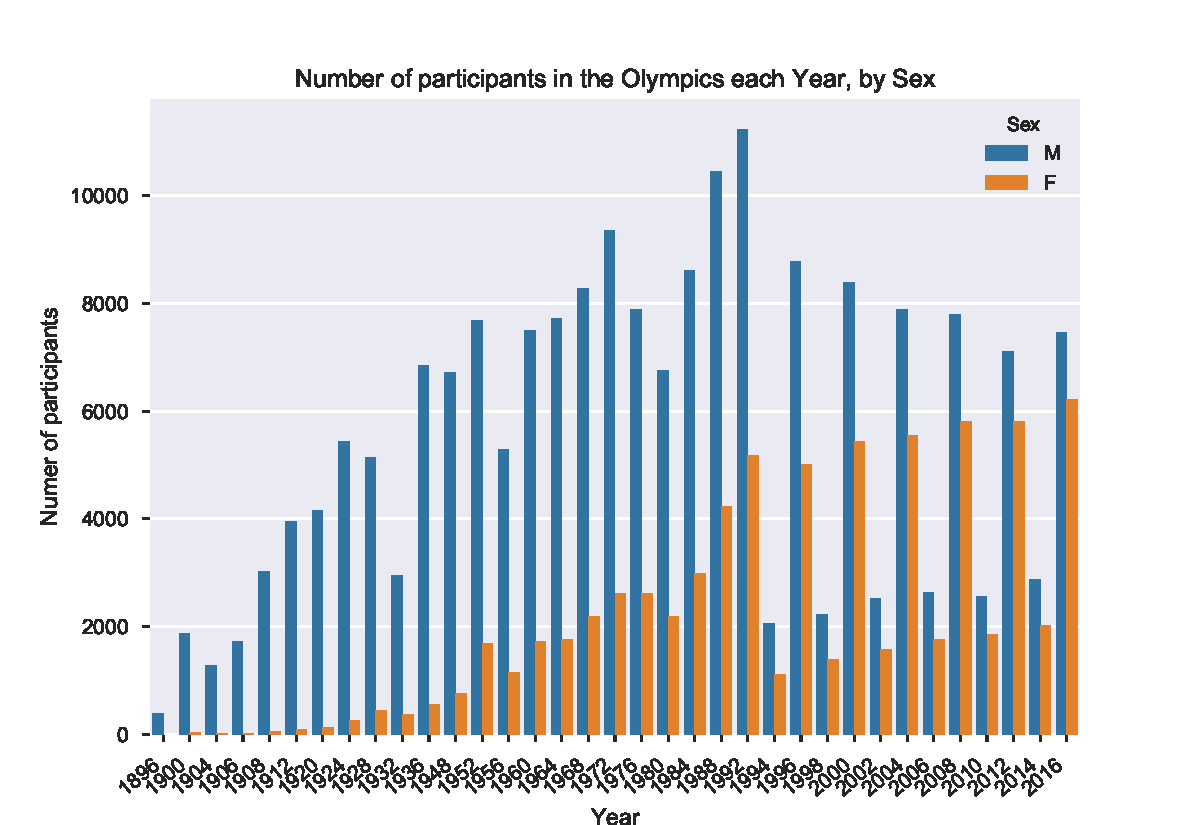
\includegraphics[scale=0.6]{Participants_year_sex.pdf}
    \caption{Comparison between women and men participation in the Olympics.}
\end{figure}

\begin{figure}
    \centering
    \begin{subfigure}{0.5\textwidth}
    \hspace{-17mm}
    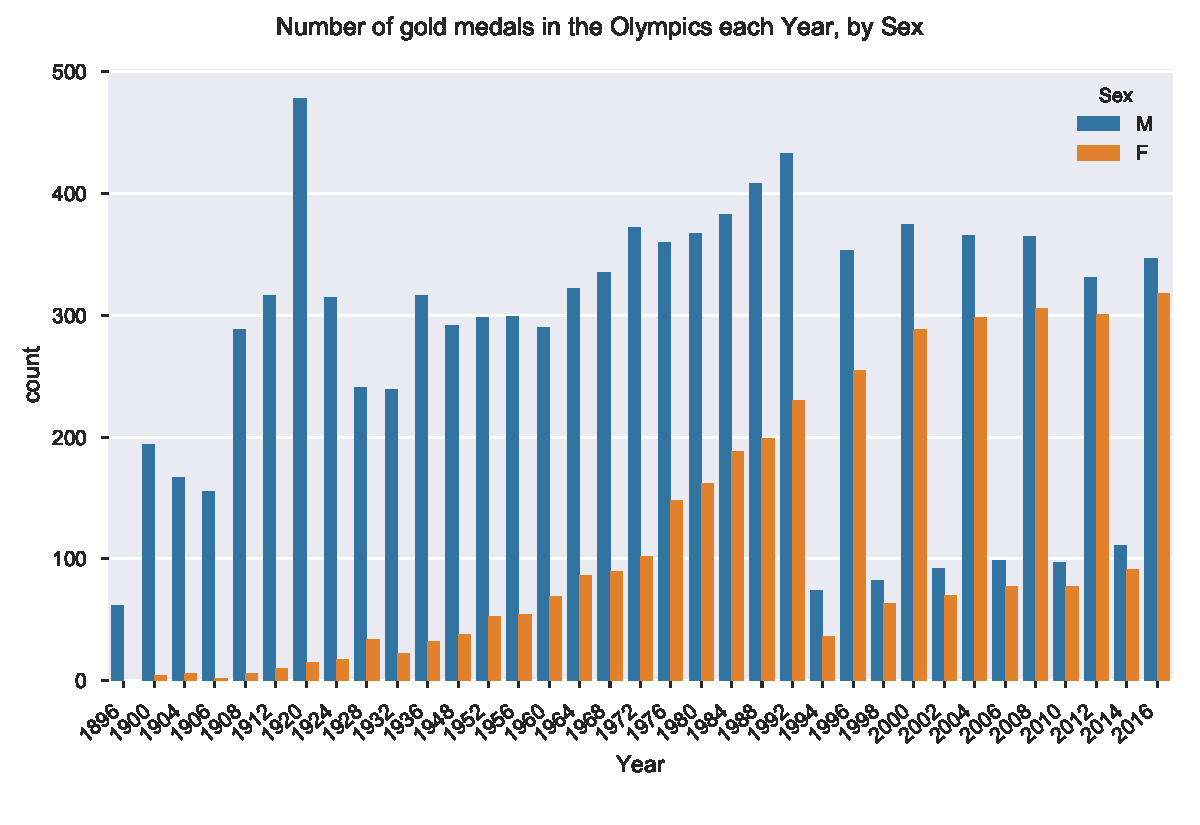
\includegraphics[scale=0.45]{Gold_year_sex.pdf}
    \end{subfigure}%
    \begin{subfigure}{0.5\textwidth}
    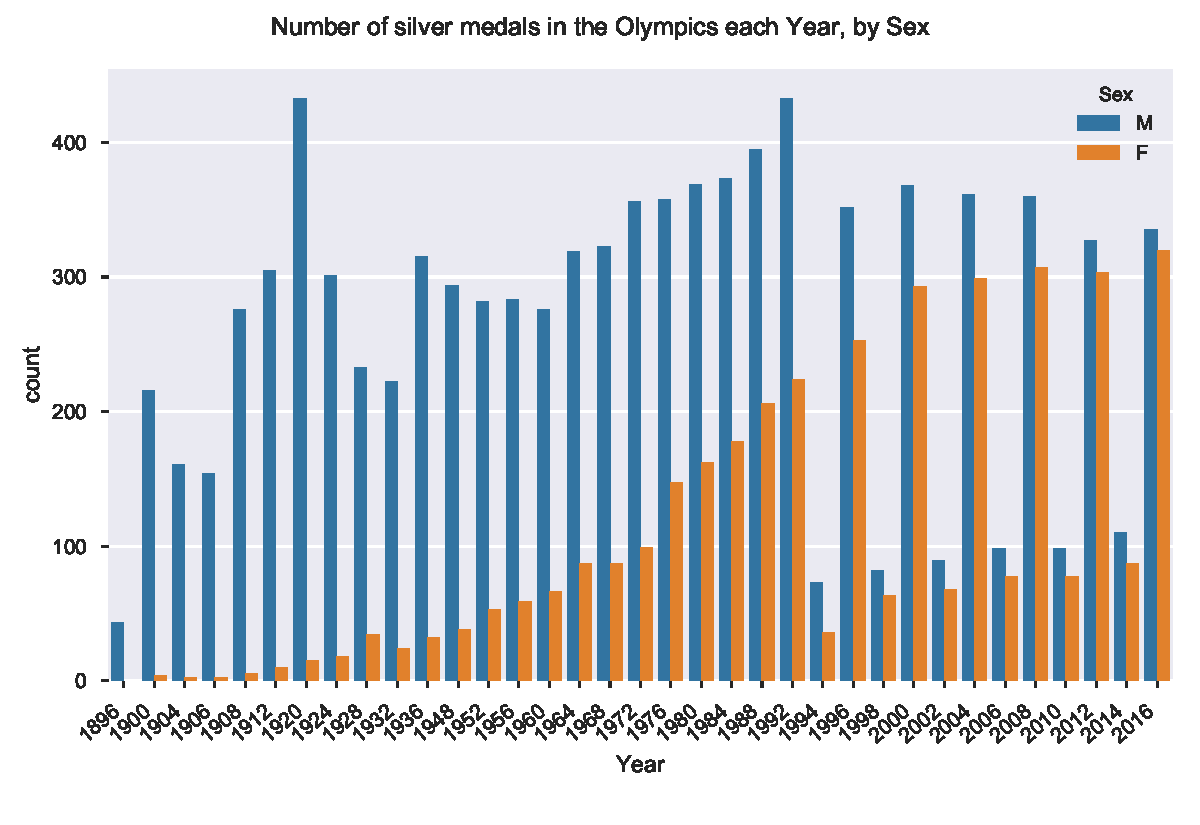
\includegraphics[scale=0.45]{Silver_year_sex.pdf}
    \end{subfigure}
    \begin{subfigure}{0.5\textwidth}
    \centering
    \hspace{-10mm}
    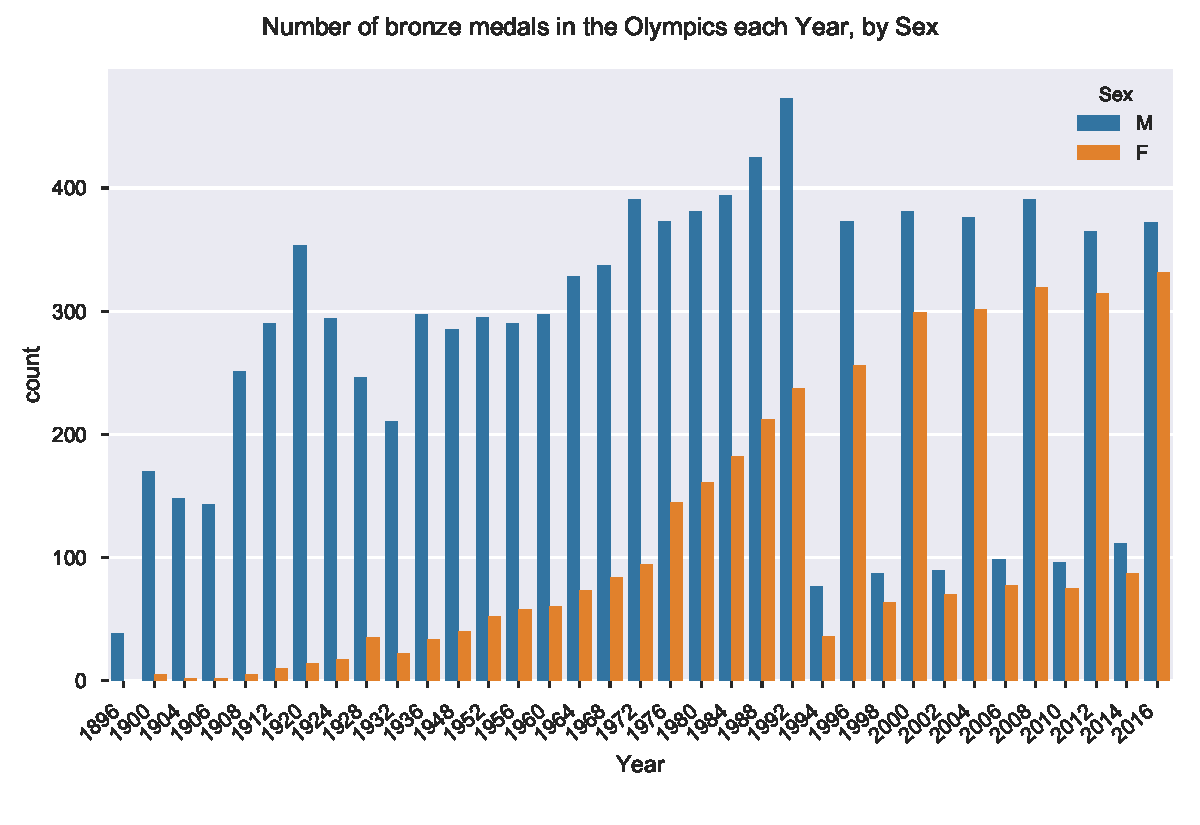
\includegraphics[scale=0.45]{Bronze_year_sex.pdf}
    \end{subfigure}
    \caption{Number of medals for women and men in the Olympics Games since 1896.}
\end{figure}

\begin{figure}
    \centering
    \begin{subfigure}{0.5\textwidth}
    \hspace{-23mm}
    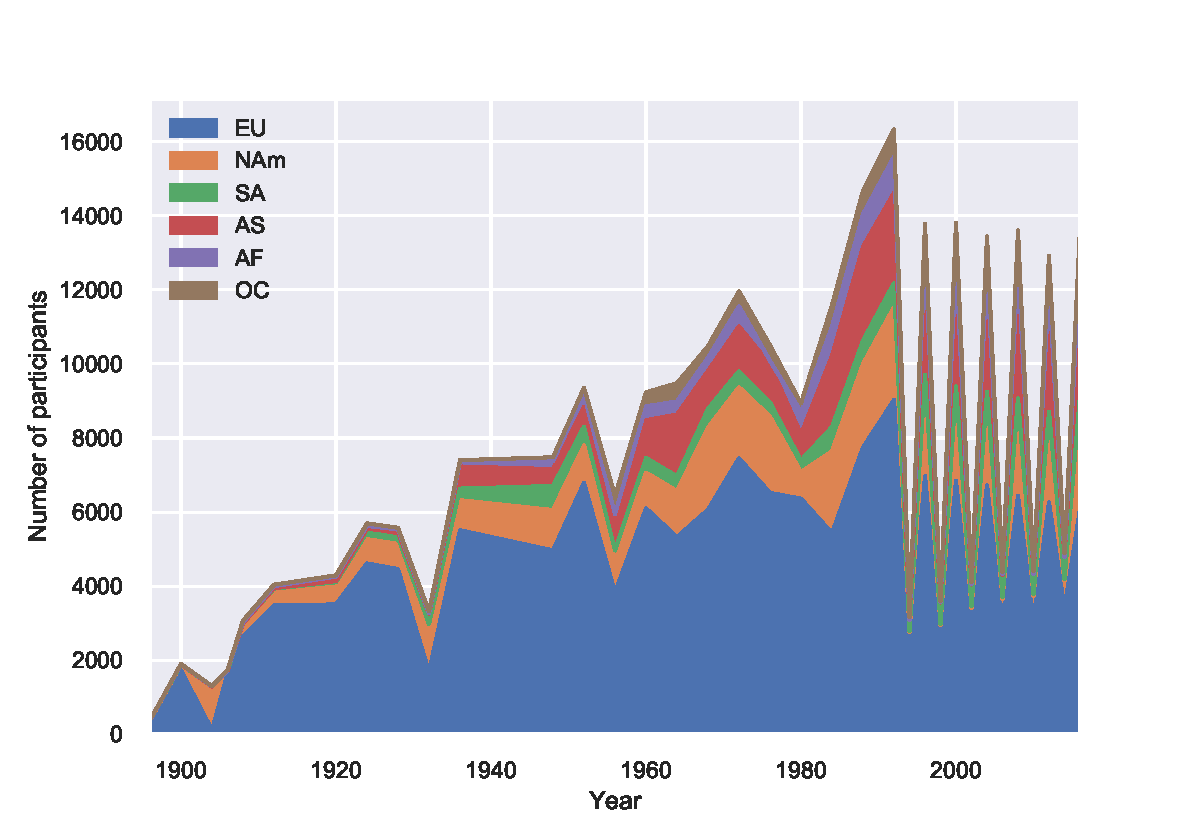
\includegraphics[scale=0.5]{Continent_area.pdf}
    \subcaption{Participants in the Olympics by Continent.}
    \end{subfigure}%
    \begin{subfigure}{0.5\textwidth}
    \centering
    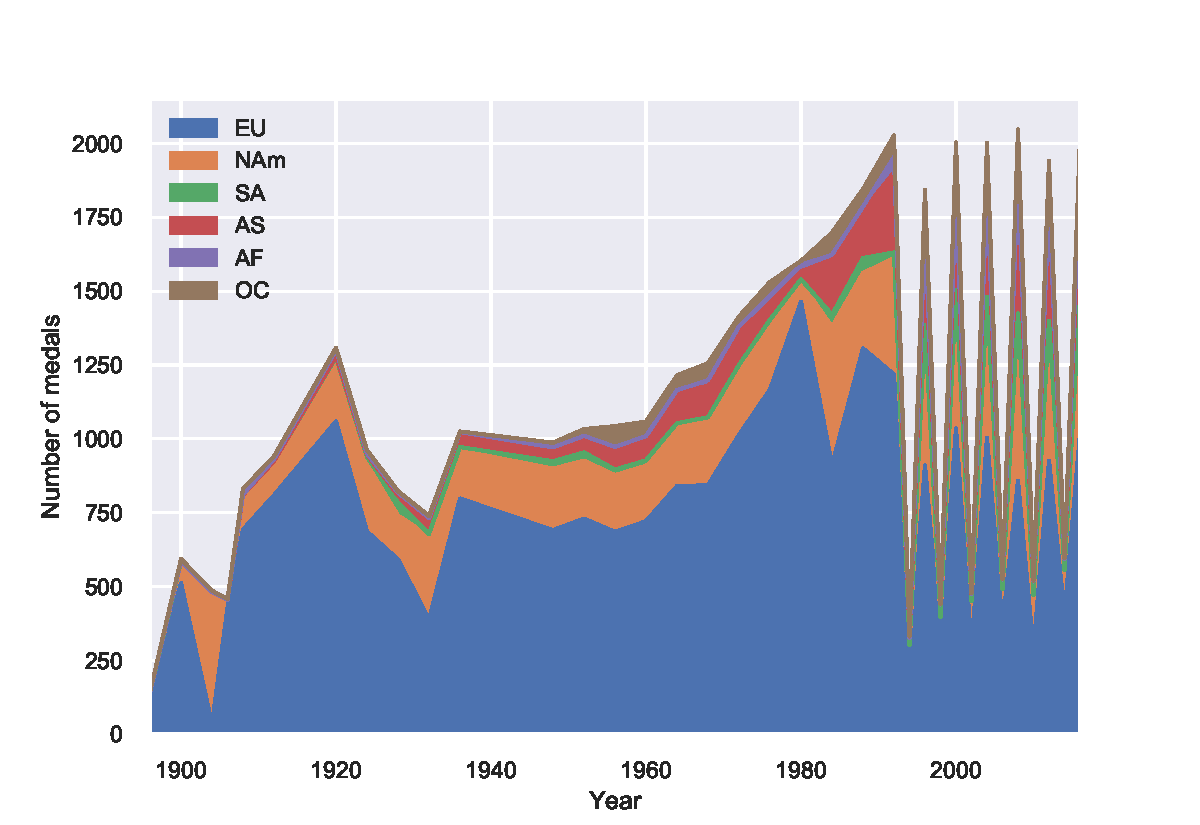
\includegraphics[scale=0.5]{Continent_area_medals.pdf}
    \subcaption{Medalists in the Olympics by Continent.}
    \end{subfigure} 
    \caption{Athletes and medals.}
\end{figure}

\begin{table}
\centering
\begin{tabular}{lrrrrrrrr}
\toprule
Continent  &EU    & NAm   & SA    & AS    & AF    & OC    &  Multi & UNK   \\
\midrule
Medal Proportion  &          0.16 &          0.20 &          0.08 &          0.10 &          0.05 &          0.15 &          0.05 &          0 \\
\bottomrule
\end{tabular}
\caption{Proportion of medalists among different continents.}
\end{table}

This observation leads us to the question of which country has been awarded more medals over the years. Here it would perhaps be relevant to have a separation between Summer and Winter Games, given that countries with different climatic conditions could be prone to performing better at certain sports promoted by those conditions. These considerations lead us to Figures 14 and 15. In first place, there is a difference between the number of participations in Summer and Winter Games, with Canada going up to third place in the Winter, as opposed to eighth place. Nordic countries (Norway, Sweeden) together with Austria and Switzerland figure in the Winter chart, but not on the Summer chart. The same behaviour can be observed in the medals, Figure 15, where Nordic countries, this time including Finland, appear in the top medalists. It is also noteworthy that in the Winter Games, Russia has more medals than the USA, as opposed to the Summer Games, where the USA lead by a wide margin. In medals, the UK figures in fourth place for the Summer Games, dropping out of the chart in the Winter ones, leaving space for Canada to take up its place. In summary, the observed results corroborate the initial hypothesis that countries would perform differently in different seasons of the Olympics.

\begin{figure}
    \centering
    \begin{subfigure}{0.5\textwidth}
    \hspace{-17mm}
    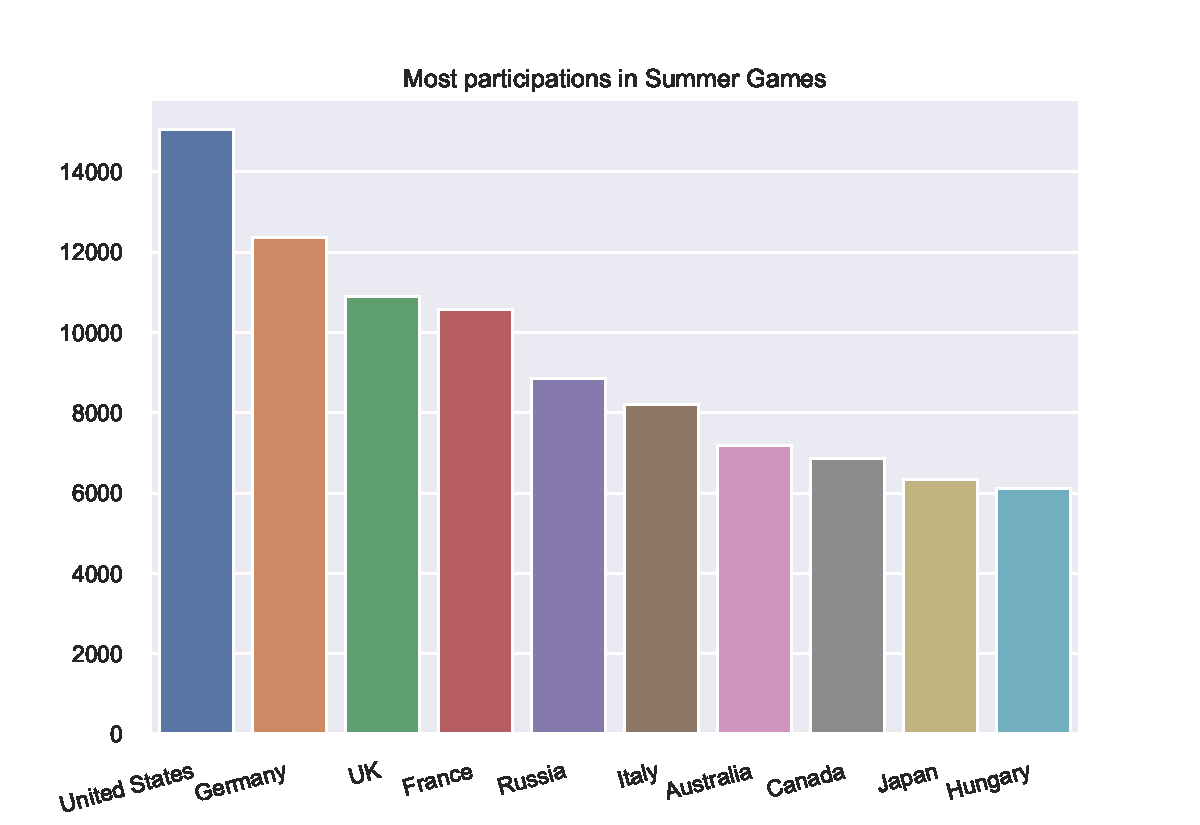
\includegraphics[scale=0.45]{Most_part_summer_countries.pdf}
    \end{subfigure}%
    \begin{subfigure}{0.5\textwidth}
    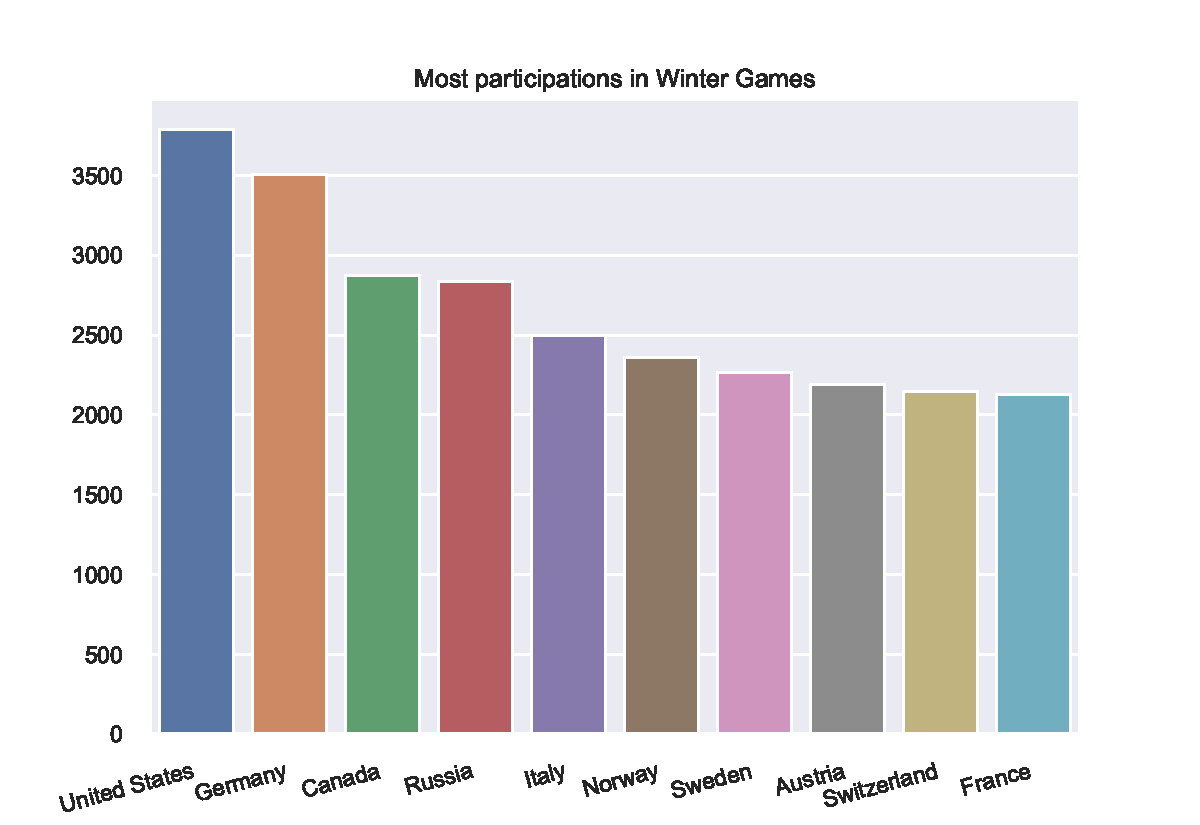
\includegraphics[scale=0.45]{Most_part_winter_countries.pdf}
    \end{subfigure}
    \caption{Countries with the most participations in the Games.}
\end{figure}

\begin{figure}
    \centering
    \begin{subfigure}{0.5\textwidth}
    \hspace{-17mm}
    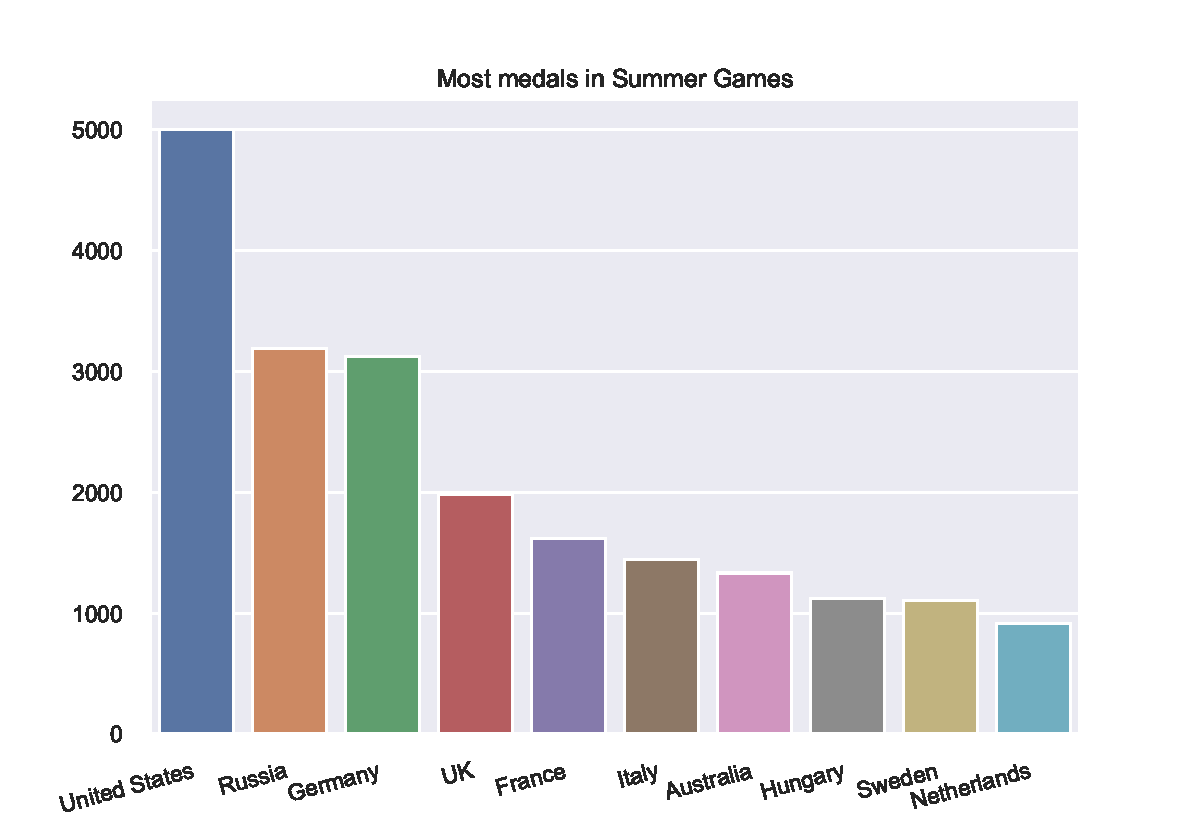
\includegraphics[scale=0.45]{Most_medals_summer_countries.pdf}
    \end{subfigure}%
    \begin{subfigure}{0.5\textwidth}
    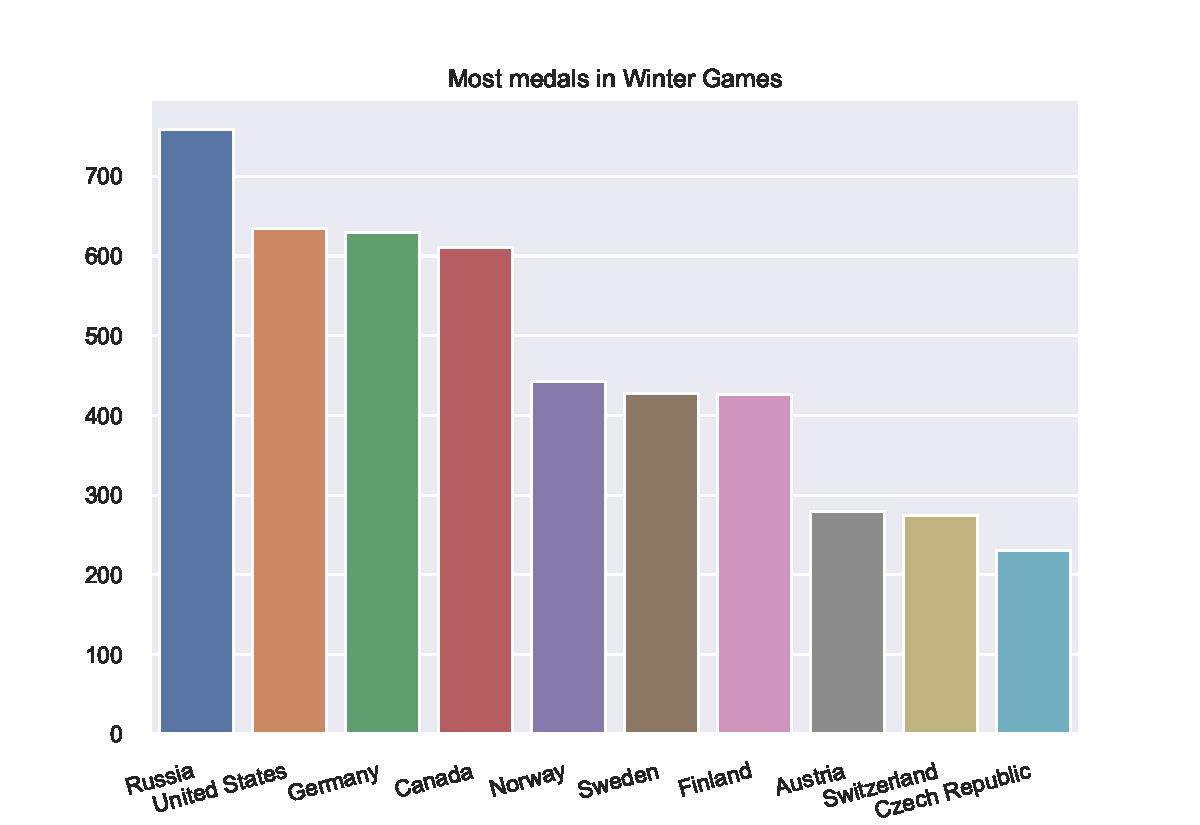
\includegraphics[scale=0.45]{Most_medals_winter_countries.pdf}
    \end{subfigure}
    \caption{Countries with the most medals in the Games.}
\end{figure}

\section{Summary and Conclusions}

In this document a brief but, in my view, robust and exhaustive report was made, on the "Olympic History" dataset from Kaggle. Many aspects were explored, such as the Age, Height and Weight distributions, the outliers in the "Age" variable were further explored, giving rise to the revelation of the existence of Art Competitions in the Olympics as many of the participations and medals awarded to people over 50 were in this category. Then, a brief exploration was made on the participants younger than 15, were it was concluded to be mostly female participants in swimming and gymnastics. Through the use of histograms, it was seen that the categorical variables "Sex" and "Sport" had influence over the distributions of the numeric variables "Age", "Height" and "Weight", as opposed to the variable "Medal" which seemed to have little impact. The relationship between "Height" and "Weight" was also analysed through a scatterplot and a strong correlation was found and corroborated through the plotting of the correlation matrix.

A time analysis was then performed, to see how the number of participants had evolved over time, having been concluded that it only decreased mostly because of political boycotts to the Olympics. It was also seen that the number of women participating has increased dramatically over the years, and that currently almost half the athletes are female. It was also seen that it was in 1992 that the Summer and Winter Olympic games were split in different years.

When analysing the data having into consideration the continent and country several insights were made. First, the most represented continent in the Olympic Games though the years have always been Europe, followed by North America. However, if we take the proportion of medalists to total athletes by continent, it is actually North America who has the upper hand, Europe and Oceania following in second and third, respectively. When analysing the number of participants and medals awarded by country, it was observed that the distribution varies significantly from Summer to Winter Games, with countries in colder climates, such as Canada, Switzerland and Nordic Countries, faring far better in the Winter.

In spite of this broad analysis, many further investigations could have been made. For example, investigate why are there many outliers in "Height" and "Weight" variables. This can be due to Basketball or Weightlifting, but it is difficult to be sure, without a proper analysis. Additionally,the relationship between "Age" and "Height" or "Weight" could have been studied, together with the outliers that don't follow the trend in the "Height"-"Weight" relationship. Or even how these relationships change when only gold medalists are included. Or also the distribution of medals by sport or even specific events. One could also study the evolution of "Age", "Height" and "Weight" over the years, with respect to "Season" or "Sex". It would also be possible to focus on specifi records such as the most appearences in the Olympics (person or country), or the most gold medals any person has won. It could even be studied how certain sports were taken out of the Games only to be reintroduced again lates. However, since there is so much to cover and time is finite, I tried to choose some aspects of the games I though were more relevant and interesting to analyise. All thes ideas can be further explored in a future analysis of this dataset, if the opportunity arises.































\end{document}

